The RXValid module reads in the data associated with a new frame a
byte at a time, and compares the destination MAC address to the
broadcast, multicast, and self-mac addresses. If the control inputs
allow for reception of the recovered MAC address, \signal{DESTOK} is
asserted. 

\begin{figure}
\label{rxvalid}
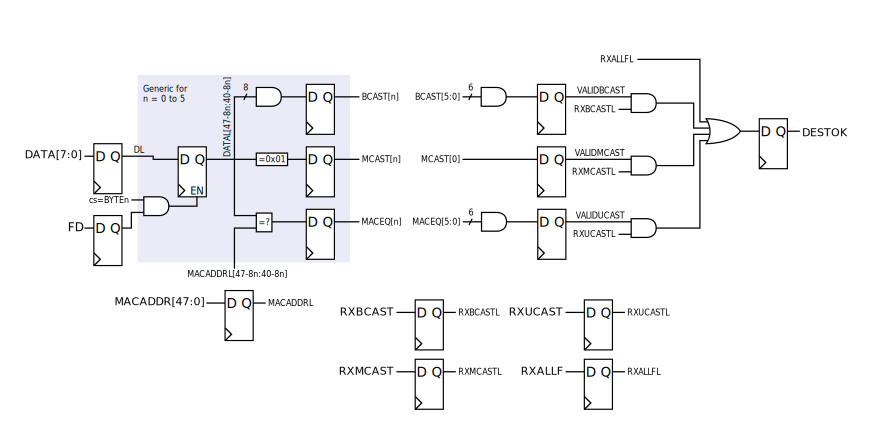
\includegraphics[scale=0.7]{rxvalid.svg}
\caption{The RX Valid Interface, verifying correct packets}

\end{figure}

\begin{figure}
\label{rxvalidfsm}
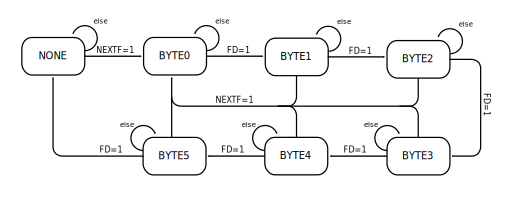
\includegraphics[scale=0.7]{rxvalid.fsm.svg}
\caption{The RX Valid FSM, verifying correct packets}
\end{figure}

